%%%%%%%%%%%%%%%%%%%%%%%%%%%%%%%%%%%%%%%%%%%%%%%%%%%%%%%%%%%
%                                                         %
% CHAPTER 04:                                             %
% The 6-electrons system                                  %
%                                                         %
% This file is part of a BSc Thesis Project. See the      %
% LICENSE file for more information about licensing.      %
%                                                         %
% Author:     Matteo Seclì <secli.matteo@gmail.com>       %
% A.Y.:       2014/2015                                   %
% URL:        https://github.com/matteosecli/QMC          %
%                                                         %
%%%%%%%%%%%%%%%%%%%%%%%%%%%%%%%%%%%%%%%%%%%%%%%%%%%%%%%%%%%

\graphicspath{{Mainmatter/figures/PNG/}{Mainmatter/figures/PDF/}{Mainmatter/figures/}}

\chapter{The 6-electrons system}

\begin{figure}[H]
	\centering
	\definecolor{myblue}{rgb}{0,0.447,0.741}	
	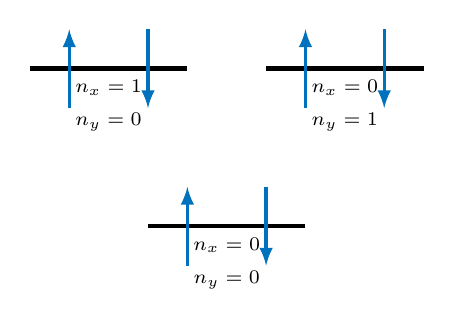
\begin{tikzpicture}
		\tikzset{>=latex}
		
		%0,0
		\draw [ultra thick] (-1,0) -- (1,0) node[midway,below,align=center] {\scriptsize $n_x=0$ \\ \scriptsize $n_y=0$};
		\draw [very thick, myblue, ->] (-0.5,-0.5) -- (-0.5,0.5);
		\draw [very thick, myblue, ->] (0.5,0.5) -- (0.5,-0.5);
		
		%1,0
		\draw [ultra thick] (-2.5,2) -- (-0.5,2) node[midway,below,align=center] {\scriptsize $n_x=1$ \\ \scriptsize $n_y=0$};
		\draw [very thick, myblue, ->] (-2,1.5) -- (-2,2.5);
		\draw [very thick, myblue, ->] (-1,2.5) -- (-1,1.5);
		
		%0,1
		\draw [ultra thick] (0.5,2) -- (2.5,2) node[midway,below,align=center] {\scriptsize $n_x=0$ \\ \scriptsize $n_y=1$};
		\draw [very thick, myblue, ->] (1,1.5) -- (1,2.5);
		\draw [very thick, myblue, ->] (2,2.5) -- (2,1.5);
	\end{tikzpicture}
	\caption{The 6-electrons system configuration.}
	\label{eq:sketch_6e}
\end{figure}

The formulae discussed in the previous sections can be generalized for a $N$ electrons case. The trial wave function can be written as
\begin{equation}
	\psi_T(\vec{r}_1 \dots \vec{r}_N)= A \,  \text{Det}(S) \prod_{i<j}^N e^{\frac{r_{ij}}{1+\beta r_{ij}}},
\end{equation}
where $\text{Det}(S)$ is the Slater determinant
\begin{equation}
	\text{Det}(S)= \left|
	\begin{matrix}
		\phi_1(\vec{r}_1) & \phi_2(\vec{r}_1) & \dots & \phi_N(\vec{r}_1) \\
		\phi_1(\vec{r}_2) & \phi_2(\vec{r}_2) & \dots & \phi_N(\vec{r}_1) \\
		\vdots &  &  & \vdots \\
		\phi_1(\vec{r}_N) & \phi_2(\vec{r}_N) & \dots & \phi_N(\vec{r}_N) \\
	\end{matrix}
	\right|
\end{equation}

As we did in Section \ref{sec:considerations}, this determinant can be further simplified if we label our electrons in a smart way, as shown in \cite{Hjorth-Jensen2014}.

Let's consider a spin-independent quantum mechanical operator $\hat{O}(\vec{r}) $ acting on our trial wave function. The latter depends on $\vec{x} = (\vec{r}, \sigma) $ where $\vec{r}$ includes the space coordinates and $\sigma$ the spin coordinates.
We have that:
\begin{equation}
	\Braket{\hat{O}} = \frac{\Braket{\psi_T(\vec{x})|\hat{O}(\vec{r})|\psi_T(\vec{x})}}{\Braket{\psi_T(\vec{x})|\psi_T(\vec{x})}}
\end{equation}

Now we can replace the total antisymmetric wave function with one with permuted arguments and we can arbitrarily choose that the first $N/2$ arguments are spin up and the other half are spin down. We get:
\begin{align}
	\psi_T(\vec{x_1},\ldots,\vec{x_N}) 
	\longrightarrow& \, \psi_t(\vec{x_{i1}},\ldots,\vec{x_{iN}}) \\
	=& \, \psi_T(\{\vec{r_{i1}}, \uparrow\},\ldots,\{\vec{r_{iN/2}}, \uparrow\},\{\vec{r_{i1}}, \downarrow\},\ldots,\{\vec{r_{iN/2}}, \downarrow\}) \\
	=& \, \psi_T(\{\vec{r_{1}}, \uparrow\},\ldots,\{\vec{r_{N/2}}, \uparrow\},\{\vec{r_{N/2 +1}}, \downarrow\},\ldots,\{\vec{r_{N}}, \downarrow\})
\end{align}
The operator $\hat{O}$ is symmetric with the respect to the exchange of labels in a pair of particles, so:
\begin{equation}
	\Braket{\hat{O}} = \frac{\Braket{\psi_T(\vec{r})|\hat{O}(\vec{r})|\psi_T(\vec{r})}}{\Braket{\psi_T(\vec{r})|\psi_T(\vec{r})}}
\end{equation}

The wave function is now antisymmetric with respect to exchange of spatial coordinates of pairs of spin-up or spin-down electrons. Therefore, for spin-independent Hamiltonians, the Slater determinant can be splitted in a product of two Slater determinants, one for the single particle orbitals with spin up and the other with single particle orbitals with spin down. We have then:
\begin{equation}
	\psi_S = S^{\uparrow}S^{\downarrow}
\end{equation}
where
\begin{equation}
	S^{\uparrow} = \left|
	\begin{matrix}
		\phi_1(\vec{r}_1) & \phi_2(\vec{r}_1) & \dots & \phi_{N/2}(\vec{r}_1) \\
		\phi_1(\vec{r}_2) & \phi_2(\vec{r}_2) & \dots & \phi_{N/2}(\vec{r}_1) \\
		\vdots &  &  & \vdots \\
		\phi_1(\vec{r}_{N/2}) & \phi_2(\vec{r}_{N/2}) & \dots & \phi_{N/2}(\vec{r}_{N/2}) \\
	\end{matrix}
	\right|
\end{equation}
and  $S^{\downarrow}$ is obviously defined in a similar way. The $\phi_i$'s functions are just as the one defined in equation (\ref{eq:phi_qnums}).

So, our final trial wave-function is just
\begin{equation}
	\psi_T = |S^{\uparrow}||S^{\downarrow}|J
\end{equation}
being $J$ the Padé-Jastrow factor.

The C++ implementation of $\psi_S$ is therefore straightforward and it is shown below.

\begin{lstlisting}[language=cpp]
	double Orbitals::SlaterD(mat& r) {
	    mat D_up(n_half,n_half), D_down(n_half,n_half);
	
	    for (int i = 0; i < n_half; i++) {
	        this->set_qnum_indie_terms(r, i);
	        for (int j = 0; j < n_half; j++) {
	            D_up(i,j) = this->phi(r, i, j);
	        }
	    }
	
	    for (int i = 0; i < n_half; i++) {
	        this->set_qnum_indie_terms(r, i+n_half);
	        for (int j = 0; j < n_half; j++) {
	            D_down(i,j) = this->phi(r, i+n_half, j);
	        }
	    }
	
	    double slater = det(D_up)*det(D_down);
	
	    D_up.reset();
	    D_down.reset();
	
	    return slater;
	}
\end{lstlisting}


\section{$\omega = 0.28$}

We start by studying our system for $\omega = 0.28$. A preliminary and very rough result is shown in Figure \ref{fig:6e-028-rep}.
\begin{figure}[h]%[H]
	\centering
	\includegraphics[width=\textwidth]{6e-028-rep}
	\caption{The variational energy versus the variational parameters $\alpha$ and $\beta$. The settings used are: importance sampling with $\Delta t = 0.1$, Jastrow factor, parallelization (8 threads), $8$ variations of $\alpha$ and $\beta$ with step $0.1$, $\SI{1e5}{}$ Monte Carlo steps. $\omega=0.28$.}
	\label{fig:6e-028-rep}
\end{figure}
Restricting to the significant region, we get the result in Figure \ref{fig:6e-028-rep_fine}.

You see that the plot is no more nice like the 2-electrons case, mainly because we didn't used enough Monte Carlo steps. The problem is that now the program has to calculate $3 \times 3$ determinants every time, so it's much slower than the previous case. To refine the result, we just doubled the number of Monte Carlo loops and restricted a little bit the variational parameters grid; taking a finer grid with more Monte Carlo cycles would have required ages, literally.

Anyway, still with this configuration, we get a result that is really near the one calculated by DMC in \cite{PedersenLohne2011}, that turns out to be $\SI{7.6001 \pm 0.0001}{\atomicunit}$.

\begin{figure}[H]
	\centering
	\includegraphics[width=\textwidth]{6e-028-rep_fine}
	\caption{The variational energy versus the variational parameters $\alpha$ and $\beta$. The settings used are: importance sampling with $\Delta t = 0.1$, Jastrow factor, parallelization (8 threads), $5$ variations of $\alpha$ and $\beta$ with step $0.1$, $\SI{2e5}{}$ Monte Carlo steps. $\omega=0.28$.}
	\label{fig:6e-028-rep_fine}
\end{figure}

A nice way to test the Slater determinant code is to turn off the electron-electron repulsion. In that case, $\psi_S$ is the \emph{exact} solution (for $\alpha = 1$). We already showed in Section \ref{sec:2e_unp} that the ground-state energy for the single electron is $E_s = \hbar\omega(n_x + n_y + 1)$. Since -- in the 6 electrons case -- we have 2 electrons with $n_x + n_y = 0$ and 4 electrons with $n_x + n_y = 1$ (See Figure \ref{eq:sketch_6e}), the total energy for the ground state is
\begin{equation}
	E_{\text{gs}} = \hbar\omega\left[2(0+1)+4(1+1)\right] = 10\omega.
\end{equation}

Turning off the repulsion results in a minimum $E_{\text{gs}} = \SI{2.7999999999999 \pm 0.0000000000002}{\atomicunit}$ for $\alpha=1$, that confirms the prediction.

\section{$\omega = 0.5$}
We repeat the same calculations with $\omega=0.5$, obtaining the results in Figure \ref{fig:6e-050-rep}.
\begin{figure}[H]
	\centering
	\includegraphics[width=\textwidth]{6e-050-rep}
	\caption{The variational energy versus the variational parameters $\alpha$ and $\beta$. The settings used are: importance sampling with $\Delta t = 0.1$, Jastrow factor, parallelization (8 threads), $10$ variations of $\alpha$ and $\beta$ with step $0.1$, $\SI{2e5}{}$ Monte Carlo steps. $\omega=0.50$.}
	\label{fig:6e-050-rep}
\end{figure}

Again, our result is pretty consistent with the one calculated by DMC in \cite{PedersenLohne2011}, that is $\SI{11.7888 \pm 0.0002}{\atomicunit}$.

\section{$\omega = 1$}

Just with the same parameters used in Figure \ref{fig:6e-050-rep} but changing the frequency to $\omega=1.00$, we have the results in Figure \ref{fig:6e-100-rep}.
\begin{figure}[H]
	\centering
	\includegraphics[width=\textwidth]{6e-100-rep}
	\caption{The variational energy versus the variational parameters $\alpha$ and $\beta$. The settings used are: importance sampling with $\Delta t = 0.1$, Jastrow factor, parallelization (8 threads), $10$ variations of $\alpha$ and $\beta$ with step $0.1$, $\SI{2e5}{}$ Monte Carlo steps. $\omega=1.00$.}
	\label{fig:6e-100-rep}
\end{figure}

Once again, our result is in very good accordance with the one calculated by DMC in \cite{PedersenLohne2011}, that is $\SI{20.1597 \pm 0.0002}{\atomicunit}$.